\chapter{Éléments théoriques sur la méthode de champ de phase}
\section{Présentation des principales méthodes de suivi et de capture d'interface}

Le traitement numérique efficace des interfaces représente un enjeu majeur de la simulation numérique tant les application faisant intervenir des interfaces sont importantes. On différencie les méthodes de suivi et de capture d'interface de part leurs philosophie différentes. En effet les méthodes de suivi d'interface sont par nature lagrangienne, ces méthodes placent des marqueurs sur l'interface qui sont suivi au cours du temps. Les méthodes de capture d'interface quant à elle suivent implicitement l'interface au travers de l'évolution d'une fonction couleur. De nombreuses méthodes existent, on présente ici les principales :
\begin{itemize}
	\item[$\bullet$] \textit{\textbf{Volume of fluid (VOF) : }} Cette méthode utilise un maillage fixe découpé en cellule représentant des volumes. On associe alors à chacune de ces cellule une fraction volumique de fluide, cette proportion est alors résolu au cours du temps et la position de l'interface peut être reconstruite. Cette reconstruction a pour désavantage de ne fournir que peu d'informations viables sur l'interface. Cette méthode reste donc peu précise et est également difficile à mettre en \oe uvre en trois dimensions.
	\item[$\bullet$] \textit{\textbf{Méthode Level-Set (LS) : }}	Cette méthode repose sur la résolution implicite de l'interface au travers de la résolution d'une fonction auxiliare dite fonction ligne de niveau, généralement la distance signée à l'interface. Cette fonction se doit d'admettre une valeur nulle à l'interface, ainsi au travers de la résolution d'une équation d'advection sur cette fonction ligne de niveau, l'interface est résolue. Cette méthode convient pour les problèmes à fort changement topologique mais présente le désavantage d'être non-conservative.
	\item[$\bullet$]\textit{ \textbf{Arbitrary Lagrangian-Eulerian (ALE) : }} La méthode repose sur une double description lagrangienne (maillage mobile) et eulérienne (maillage fixe), à chaque itération temporelle, le maillage autour de l'interface est reconstruit pour s'adapter à la forme de l'interface, ainsi chaque maille contient uniquement un fluide. L'ensemble de ces propriété rend la méthode très précise mais difficile à mettre en \oe uvre en trois dimensions.
	\item[$\bullet$]\textit{ \textbf{Front-Tracking (FT) : }} La méthode utilise des marqueurs sans masse positionné sur l'interface transporté suivant une description lagrangienne sur un maillage fixe. Cette méthode nécessite l'implémentation d'algorithme pour les cas de coalescence et rupture d'interface et possède comme désavantage de ne pas conserver la masse.
\end{itemize}








\section{Méthode d'interface diffuse}
Les méthodes de suivi d'interface présenté précédemment décrivent toute l'interface comme une discontinuité, cependant il existe un second paradigme traitant l'interface comme une zone de transition continue, on parle alors d'interface diffuse.
Dans ce second cas l'interface correspond donc à une zone transition d'épaisseur connue et maîtrisée ou cohabitent les deux phases, le traitement de l'interface est alors facilité, les gradients à l'interface étant finis. Ce concept d'interface diffuse date du XIX$^{\text{ème}}$siècle et est introduit par Van Der Walls. L'intérêt de la communauté scientifique pour cette méthode apparaît dans les années 1950 avec la description de l'énergie libre par Ginzburg et Landau et son utilisation par Cahn et Hilliard en 1958 \cite{cahn_free_1958} pour obtenir une description thermodynamique de l'interface.
\begin{figure}[H]
	\centering
	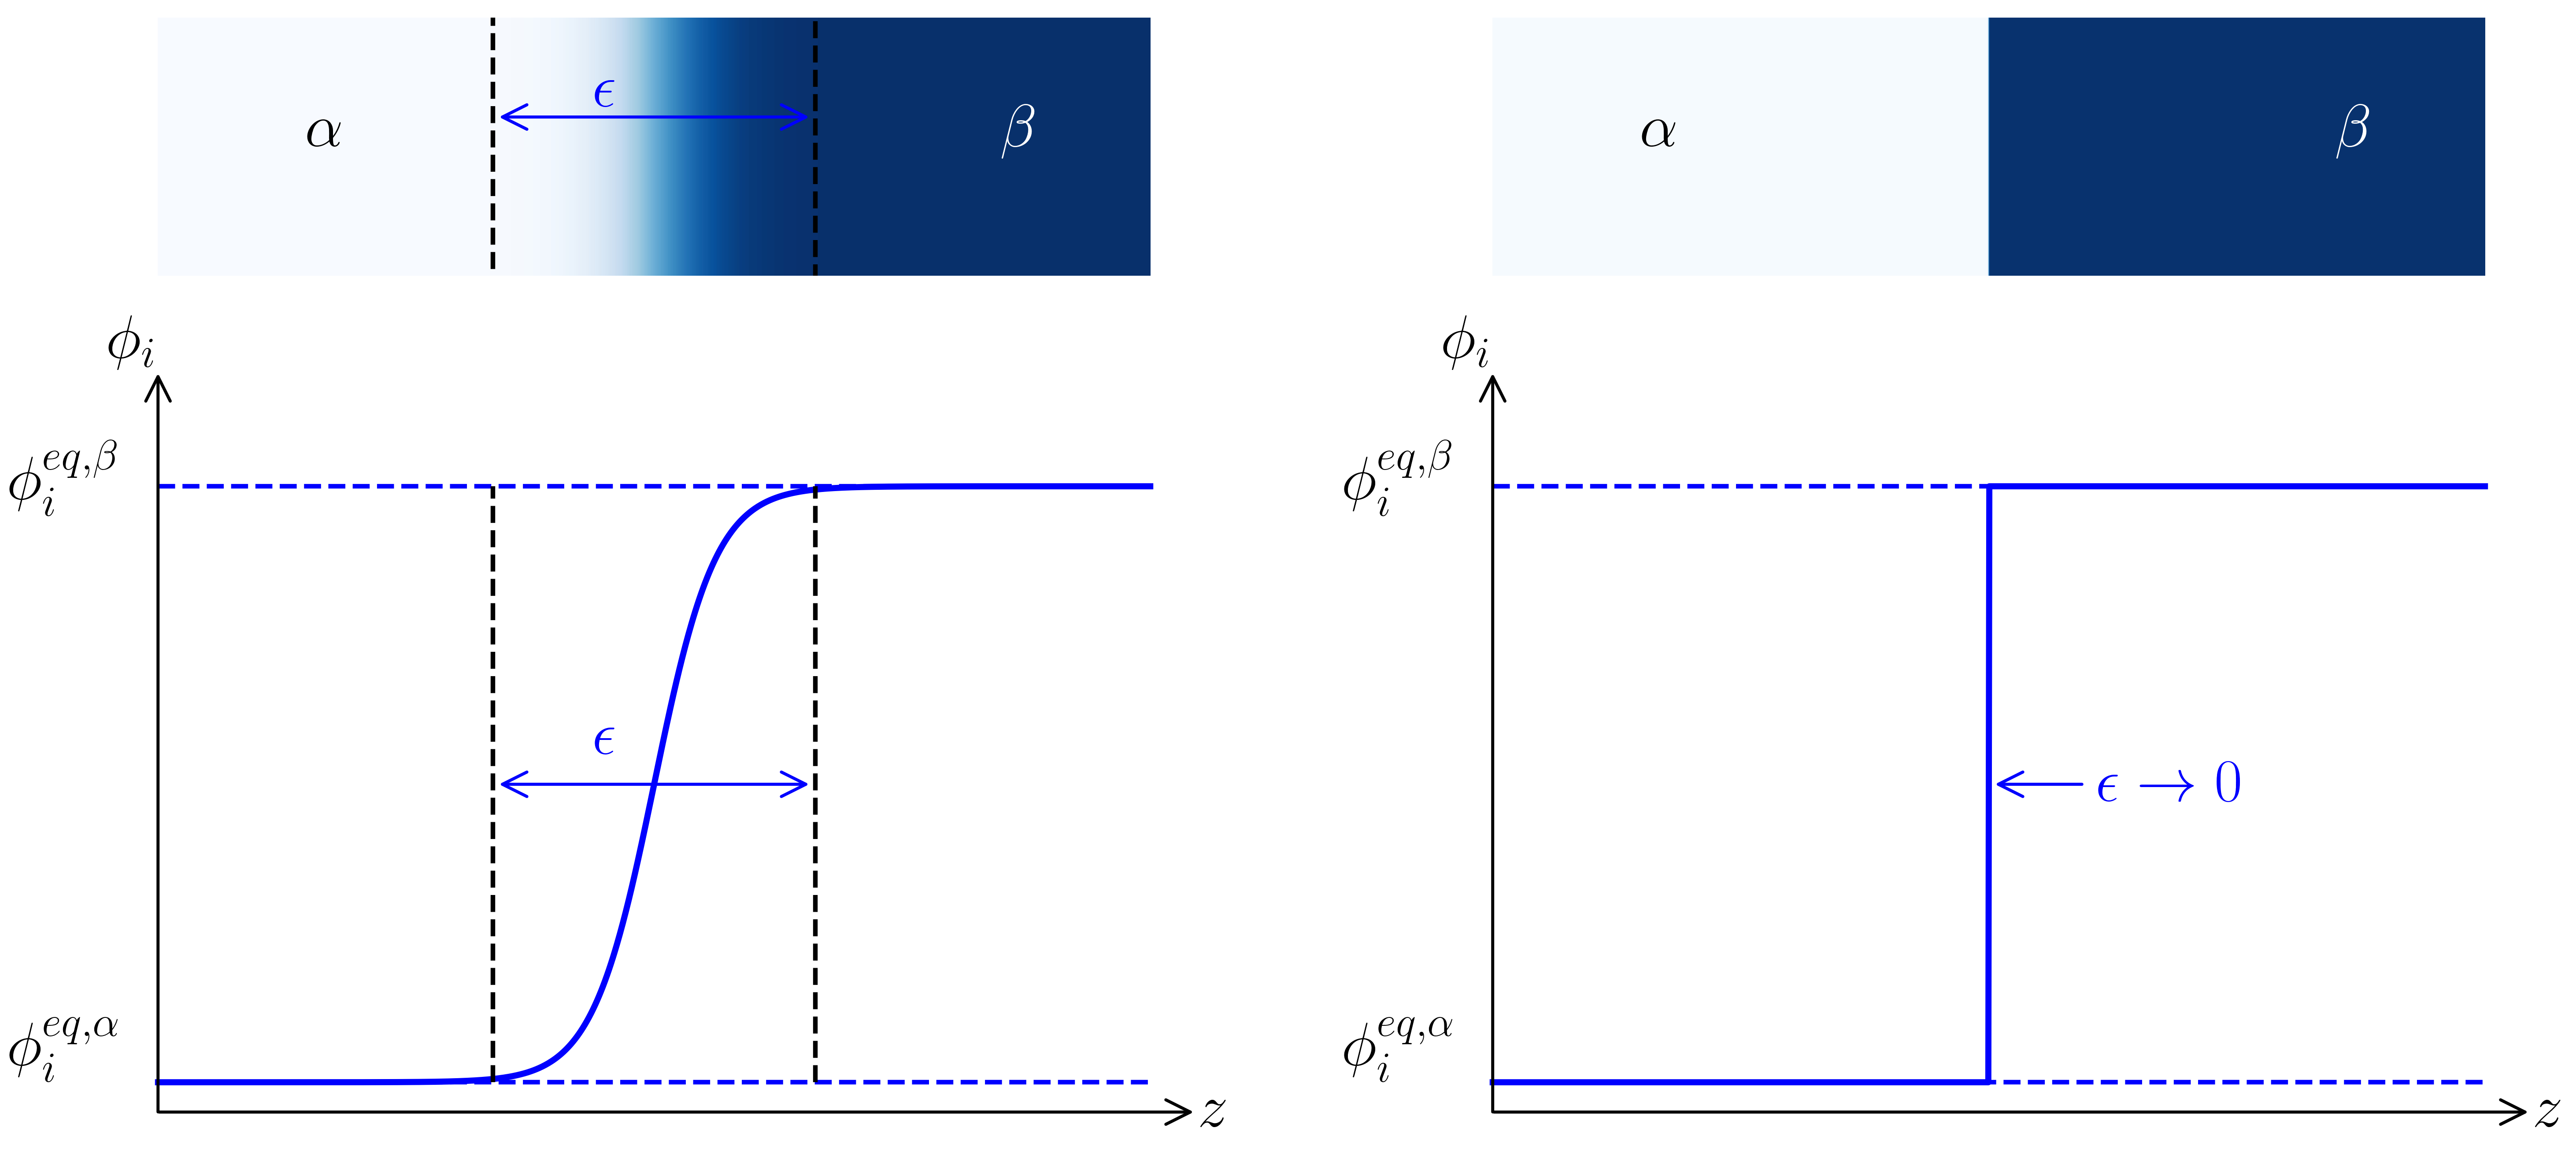
\includegraphics[width=0.7\linewidth]{figure/diffuse_interface}
	\caption{Comparaison entre une interface raide et une interface diffuse}
	\label{fig:diffuseinterface}
\end{figure} 
\noindent L'interface est alors suivie implicitement grâce à une fonction champ de phase définie à partir de grandeurs thermodynamiques au travers d'une variable champ de phase noté $\phi$. Cette méthode aujourd'hui utilisée dans de nombreux domaines très divers.
\begin{figure}[H]
	\centering
	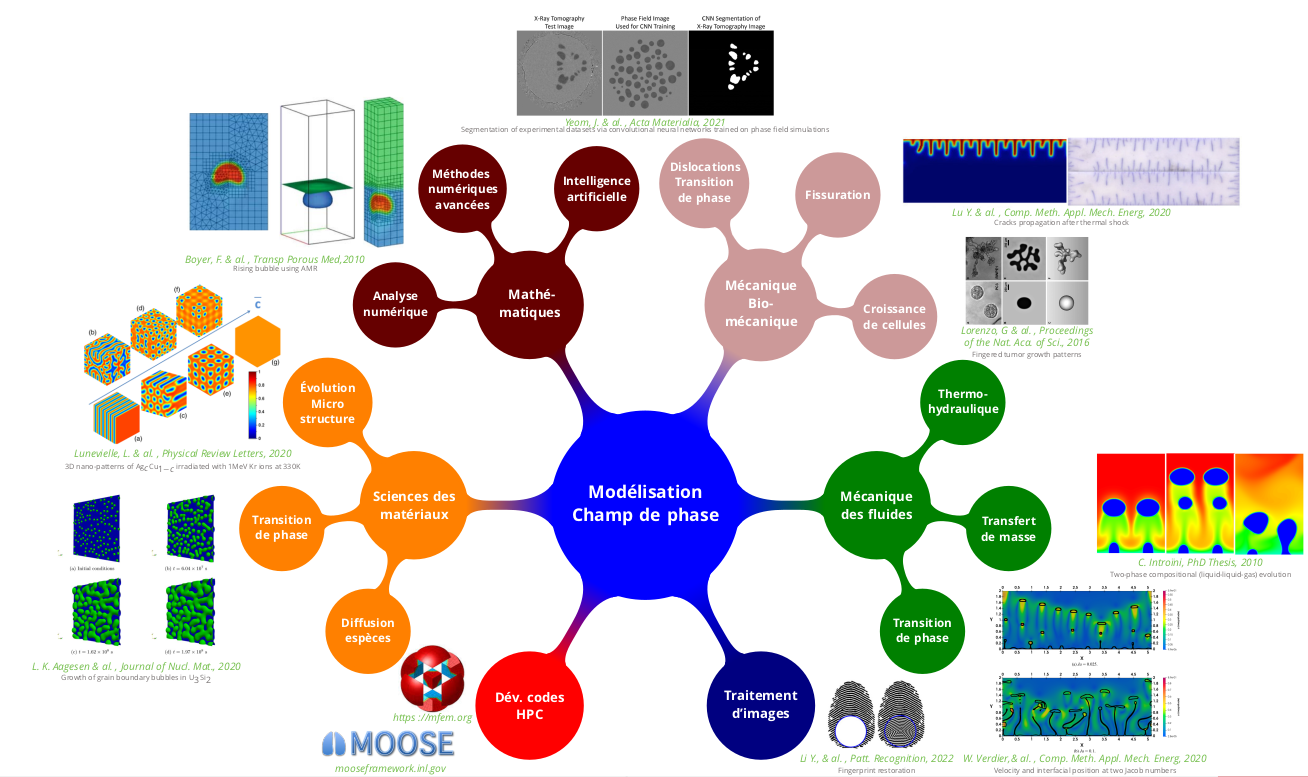
\includegraphics[width=0.9\linewidth]{figure/champ_phase}
	\caption[Domaine d'application de la méthode champ de phase]{Domaine d'application de la méthode champ de phase, tirée de \cite{introini_suivi_nodate}}
	\label{fig:champphase}
\end{figure} 
\subsection{Équation de Cahn-Hilliard généralisée}
Comme expliqué précédemment la méthode de champ de phase repose sur le suivi d'une variable de phase (ou paramètre d'ordre) noté $\phi_i$ pour le composant $i$ et contraint tel que : 
\begin{equation}
\sum_i \phi_i =1 \Rightarrow \phi_n =1 - \sum_{i=1}^{n-1} \phi_i
\end{equation} 
Ainsi pour un mélange à $n$ composants, seules $n-1$ variables sont indépendantes nécessite un suivi. Dans certains cas le système peut également être décrit avec des variables non conservées telles que des indicatrices de phases ou des grandeurs liées à des réactions chimiques, cela peut être le cas pour le dioxyde de zirconium ZrO$_2$ présent dans le corium selon les conditions initiales. Le comportement de ces variables est alors régis par des équations de réaction-diffusion dites d'Allen-Cahn, dans notre étude ce type d'équation ne sera pas résolue car l'ensemble des paramètres d'ordre sont conservés. Dans le cadre de variables conservées les équations de Cahn-Hillard pour $n$ composants, avec $i\in \{1,..,n-1 \}$ s'écrivent sous la forme :
\begin{equation}
	\cfrac{\partial \phi_i}{\partial t} + \left(\mathbf{u} \cdot \nabla\right) \phi_i =  \nabla \cdot \left(\sum_{j=1}^{n-1}{\mathcal{M}_{ij}} \nabla\left( \frac{\delta \mathbb{F}}{\delta \phi_j}\right) \right) 
\end{equation}
avec : $\mathcal{M}_{ik}$ la mobilité (paramètre cinétique),  $\phi$ le paramètre d'ordre, $\mathbf{u}$ la vitesse et $\mathbb{F}$ une fonctionnelle de Ginzburg-Landeau généralisée \cite{cardon_modelisation_2016} définit tel que : 
 \begin{equation}
\mathbb{F}[\phi_1,..,\phi_n] = \int_{\mathcal{V}}\lambda\tilde{f}_0(\bm{\phi},\mathbf{x},t)+ \sum_{i=1}^{n-1}\sum_{j=1}^{n-1}\cfrac{1}{2}\kappa_{ij}\nabla \phi_i \cdot \nabla \phi_j dV
\end{equation}
Où le premier terme représente la densité d'énergie liée aux valeurs locales de composition, traduisant l'équilibre des phases ainsi que leurs existences ou coexistence. Pour deux phases $\alpha$ et $\beta$, on rappel l'équilibre thermodynamique donné par :
\begin{subequations}
	\begin{align}
		&\left.\frac{\partial \tilde{f}}{\partial \phi_i}\right|_{\phi_i^{\alpha,eq}} = \left.\frac{\partial \tilde{f}}{\partial \phi_i}\right|_{\phi_i^{\beta,eq}} = \tilde{\mu}_i^{eq} \hspace{1cm} \Leftrightarrow   \hspace{1cm} \tilde{\mu}_i^{\alpha,eq} = \tilde{\mu}_i^{\beta,eq} \\
		& 		\tilde{f}_0^{\alpha,eq} - \sum_{i=1}^{n-1}\tilde{\mu}_i^{eq}\phi_i^{\alpha,eq} = 	\tilde{f}_0^{\beta,eq} - \sum_{i=1}^{n-1}\tilde{\mu}_i^{eq}\phi_i^{\beta,eq}
	\end{align} 
\end{subequations}
$\tilde{\mu}_i^{eq}$ représente un potentiel de diffusion de l'élément $i$ à l'équilibre.\\
Le second terme représente la contribution des interfaces, le coefficient $\kappa$, dit coefficient de gradient, tient compte du coût énergétique engendré par l'interface, par la suite ce paramètre pourra être relié à la tension de surface. \\
%Dans le cas binaire il est possible de décrire géométriquement l'ensemble des variables : 
%\begin{figure}[H]
%	\centering
%	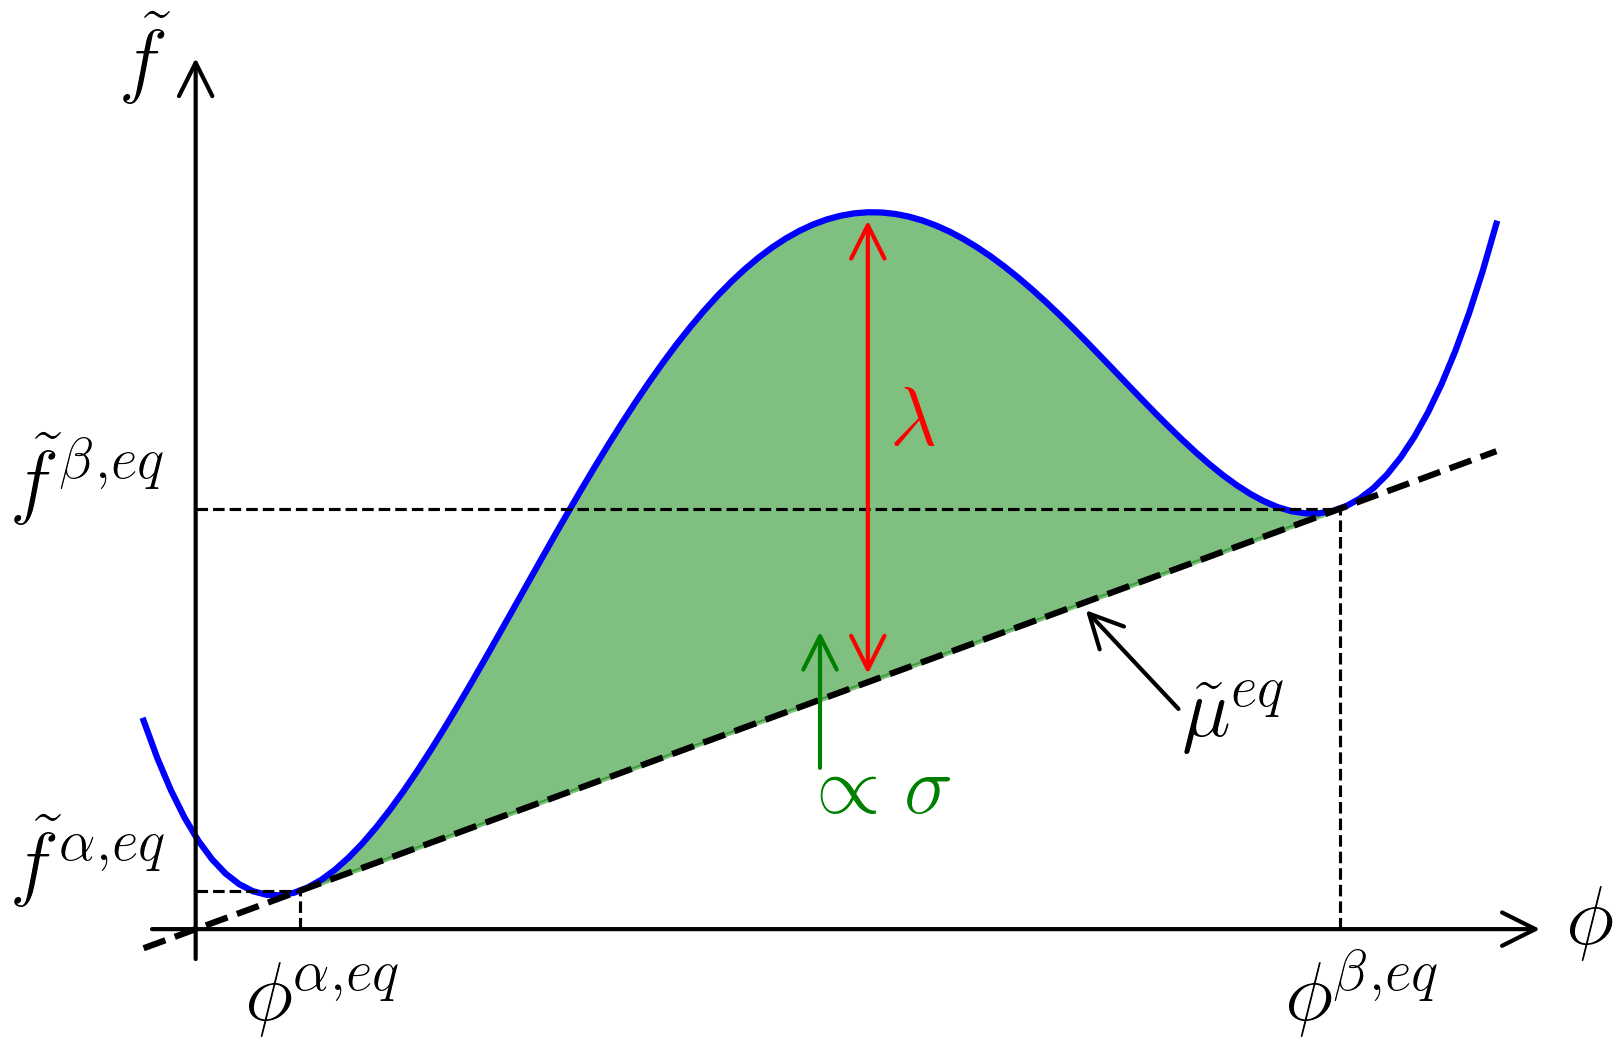
\includegraphics[width=0.45\linewidth]{figure/fig_NRJ}
%	\caption{Description de l'énergie libre pour un système binaire}
%	\label{fig:fignrj}
%\end{figure}
Finalement la dérivé variationnelle de cette fonctionnelle d'énergie libre peut être définit comme un potentiel de diffusion $\tilde{\mu}$: 
\begin{equation}\label{eq_potentiel}
	\frac{\delta \mathbb{F}}{\delta \phi_j} =\lambda \frac{\partial \tilde{f}_0}{\partial \phi_j} -\sum_{k=1}^{n-1} \kappa_{jk} \Delta \phi_k = \tilde{\mu}_j
\end{equation}
avec $\lambda$ un paramètre d'upscalling numérique ajouté pour augmenter l'épaisseur de l'interface, dans le cas où $\lambda=1$ l'interface est d'épaisseur "réelle" soit de l'ordre de l'angstr\oe m, les capacités de calcul ne permettant pas de pouvoir faire des calculs avec des maillages contenant de si petits éléments. \\
Le potentiel de diffusion peut être relier au potentiel chimique classique tel que :
\begin{equation}
	\tilde{\mu}_i = \frac{1}{V_m}\left(\mu_i - \mu_n\right)
\end{equation}
Avec $\tilde{\mu}_i$ (en J.m$^{-3}$) représente le potentiel de diffusion de l'élément $i$, et $V_m$ le volume molaire supposé constant dans tout le système.\\
%Le potentiel chimique étant classiquement définit tel que :
%\begin{equation}
%	\mu_i = \left.\frac{\partial G}{\partial n_i}\right|_{P,T,n_{j\neq i }} = \left.\frac{\partial F}{\partial n_i}\right|_{V,T,n_{j\neq i }}
%	  \textrm{                        où           } F = V_m f_0
%\end{equation}
%Avec $F$ (resp. $G$) l'énergie libre d'Helmotz (resp. Gibbs) (en J) et $n_i$ la quantité de matière de l'élément $i$ (en mol). Dans notre cas on se place dans une transformation isobare et isotherme, on privilégiera donc l'énergie de libre de Gibbs.
Dans le cas où $\doubleoverline{\kappa}$ = $\doubleoverline{0}$ on retrouve une équation d'advection-diffusion classique, dans le cas contraire on obtient une équation d'ordre 4. Une des principale difficulté dans la mise en place de méthode champ de phase repose sur le paramétrage des simulations.
\subsection{Couplage avec les équations de Navier-Stokes incompressible}
Dans le cadre de cette étude les équations de Cahn-Hilliard sont couplées aux équations de conservation de masse et de quantité de mouvement incompressible sous l'approximation de Boussinesq, d'après \cite{kim_phase-field_2012} le système d'équations s'écrit sous la forme :
\begin{subequations}
\begin{align}
&\nabla \cdot \mathbf{u} = 0\\
&\rho^* \left (\frac{\partial \mathbf{u}}{\partial t} + (\mathbf{u} \cdot {\nabla})\mathbf{u}\right) = -{\nabla} P +\eta \Delta \mathbf{u}+\sum_{i=1}^{n-1} \tilde{\mu}_i{\nabla} \phi_i + \rho(\bm{\phi}) \mathbf{g}
\end{align}
\end{subequations}
avec $\mathbf{u}$ la vitesse, $P$ la pression, $\mu_i$ le potentiel chimique du composant $i$, $\mathbf{g} = \{ 0,0,-g\}^T $, $\eta$ la viscosité cinématique supposée constante, $\rho^*$ la masse volumique du solvant \\
L'approximation de Boussinesq est utilisé pour calculé la densité dans le terme de flottabilité :
\begin{equation}
	\rho(\bm{\phi}) = \rho^*\left(1+\sum_{i=1}^{n-1}\beta_i \phi_i\right)
\end{equation}
Les paramètres $\beta_i$ sont à déterminer en fonction du système étudié, $\rho^*$ correspond à une masse volumique de référence, généralement celle du solvant. L'équation de Cahn-Hilliard étant d'ordre 4, une résolution implicite est alors préférée pour les simulations.
\subsection{Paysage thermodynamique analytique}
L'objectif présenté dans \cite{noauthor_numerical_nodate} est de d'obtenir une formulation analytique du terme homogène de la fonctionnelle de Ginzburg-Landau. Dans le cas binaire, cette contribution est de la forme d'un double puits, généralement un polynôme de degré 4 :
\begin{figure}[H]
	\centering
	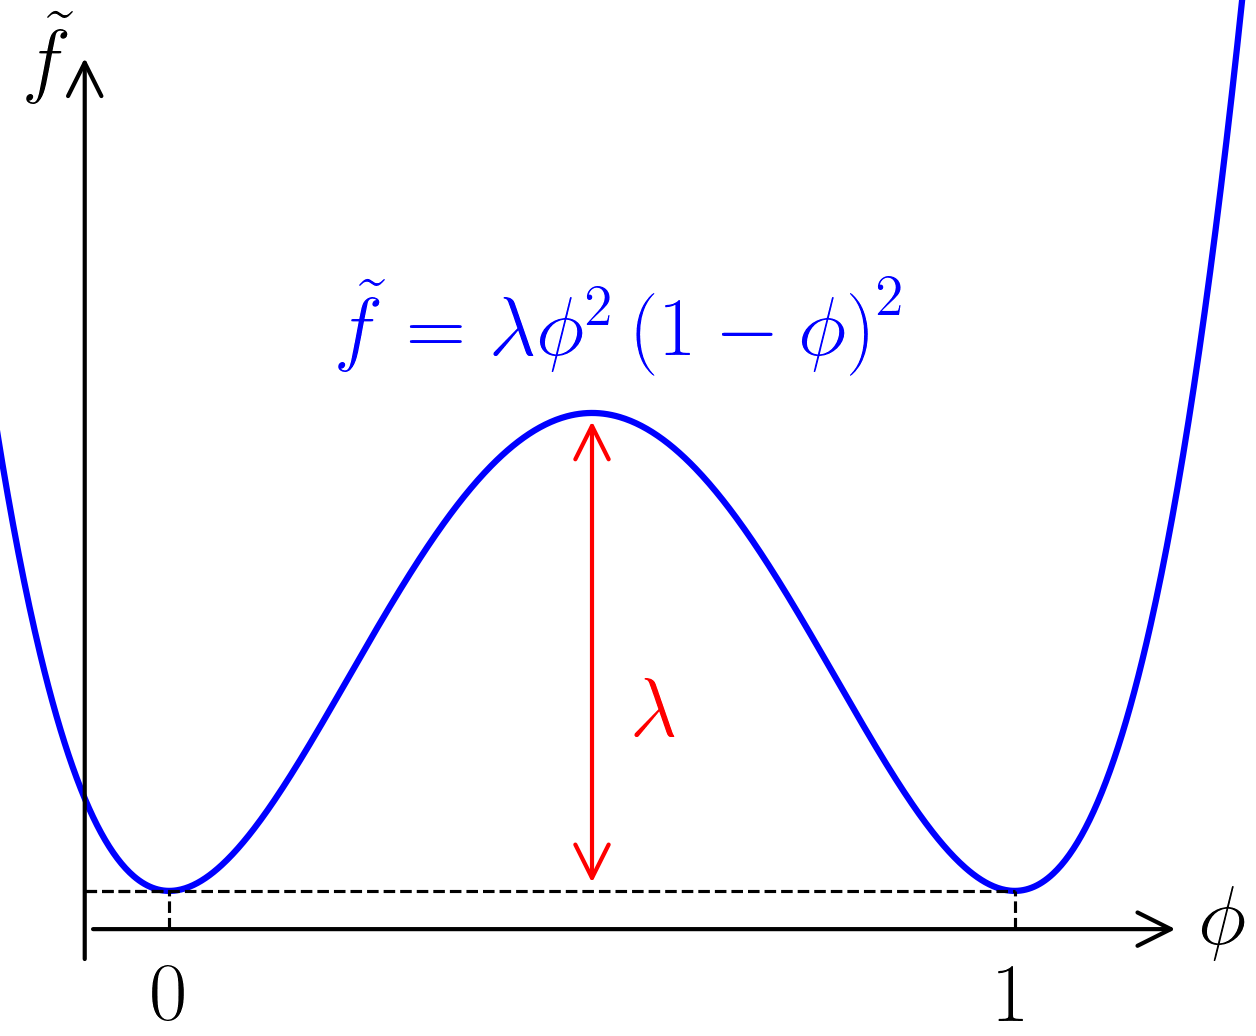
\includegraphics[width=0.3\linewidth]{figure/figpolydeg4}
	\caption{Description classique du terme homogène de la description de l'énergie pour un système binaire completement immiscible}
	\label{fig:figpolydeg4}
\end{figure}
L'objectif est de généraliser ce double puits pour un système n-aire, ainsi on introduit un pseudo grand potentiel correspondant à la hauteur énergétique nécessaire pour changer de minimum d'énergie \cite{cardon_modelisation_2016}.
\begin{equation}
\Omega^{\star} =\Omega - \Omega^{eq} =  \tilde{g}^{liq} - \sum_i \tilde{\mu}_i^{eq}\phi_i - \left(  \tilde{g}^{liq,eq} -  \sum_i \tilde{\mu}_i^{eq}\phi_i^{eq} \right) 
\end{equation}
avec $\tilde{g}^{liq}$ l'énergie libre de Gibbs, utilisé comme grandeur d'intérêt ici puisque le système est supposé isotherme et isobare.
Les bases thermodynamiques étant peu développées aux points d'intérêt (Température supérieure à 2000 \textdegree C) on cherche à définir ce potentiel grâce à une formulation analytique en double puits que l'on note :
\begin{equation}\label{double_puit}
	\Omega^{\star}  = P^{dis} \times P^{cont}
\end{equation}
Où $P^{dis}, P^{cont}$ représente deux paraboloïdes correspondant à la phase dispersée et continue. Dans le cas ternaire, avec les éléments $A$ et $B$ d'intérêt, les paraboloïdes sont de la forme : 
\begin{multline}
P^{k}=\left(\frac{\co{\theta^{k}}(\phi_{A}-\phi_{A}^{eq,k}) + \sinus{\theta^{k}}(\phi_{B}-\phi_{B}^{eq,k})}{a_{}^{k}}\right)^{2}+\\ \left(\frac{-\sinus{\theta^{k}}(\phi_{A}-\phi_{A}^{eq,k}) + \co{\theta^{k}}(\phi_{B}-\phi_{B}^{eq,k})}{b^{k}}\right)^{2}
\label{eq:paraboloid_general_}
\end{multline}
Avec $k = \{disp,cont\}$ la phase (dispersée ou continue), $a$ (resp. $b$) le demi-petit (resp. demi-grand) puits, $\theta^k$ l'angle de rotation associé au puits de la phase $k$.\\
On trace alors en exemple le cas le plus simple de paysage :
\begin{figure}[H]
	\centering
	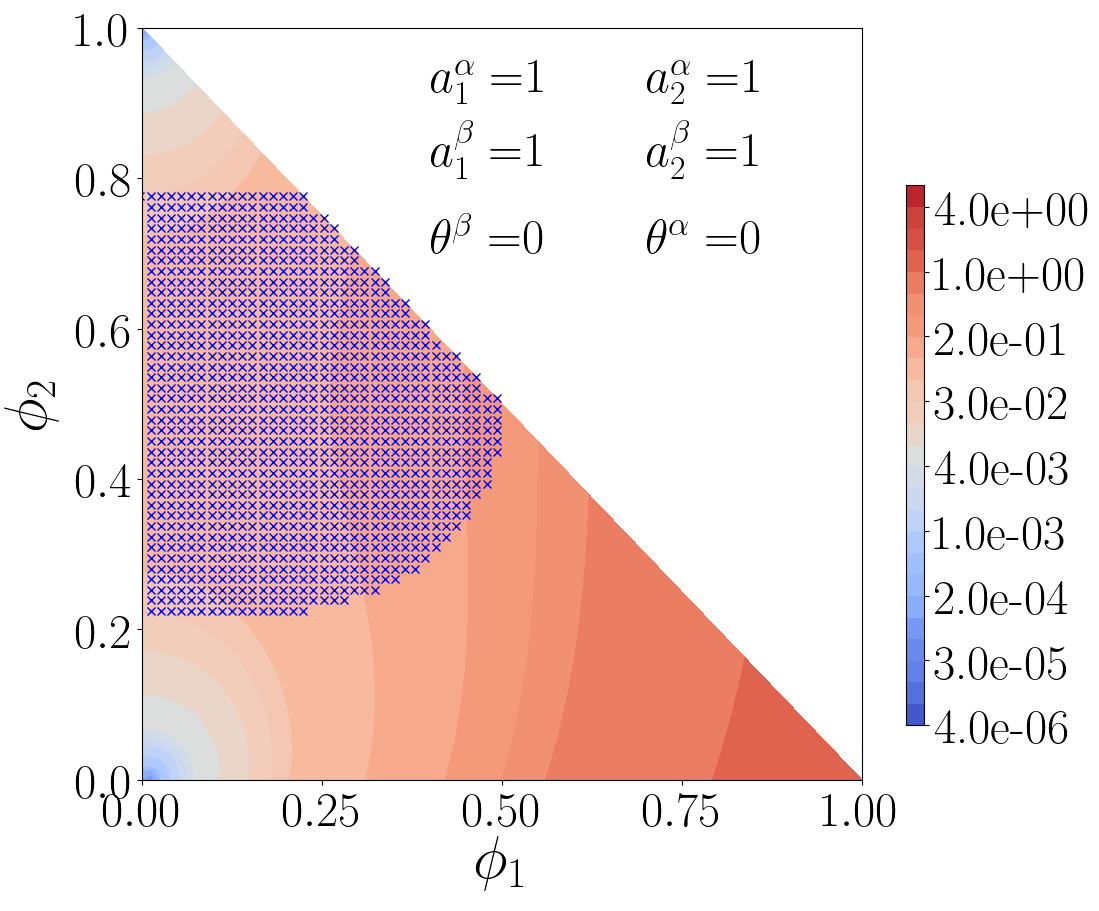
\includegraphics[width=0.6\linewidth]{figure/landscape}
	\caption{Exemple de paysage thermodynamique, la zone bleu représente la zone instable}
	\label{fig:landscape}
\end{figure}
Les éléments de calculs pour la détermination de la zone instable sont présentés en annexe \ref{ann:stabphase}. Une représentation dans le plan est possible pour le cas ternaire, pour les cas comprenant un nombre plus important de paramètre d'ordre la visualisation semble plus complexe. Ainsi cette formulation possède deux avantages, en premier lieu elle évite un couplage entre le code CFD et un solveur d'équilibre thermodynamique (Open-Calphad par exemple) réduisant significativement le temps de développement. En effet pour les cas ou le paysage est connu il est alors possible de calibrer les paramètres des paraboloïdes pour obtenir une forme analytique proche du paysage réel. Dans le cas d'un paysage inconnu, par manque d'information thermodynamique, ce paysage permet d'avoir une description cohérente pour des simulations qualitatives.
%On peut dès lors calculer le potentiel de diffusion homogène grâce à la formulation analytique (\ref{double_puit}) :
%\begin{align}
%	\tilde{\mu}_i & \nonumber= \frac{\partial}{\partial \phi_i}\left\lbrace 
%	\Omega^{\star} + \sum_j \tilde{\mu}_j^{eq}\phi_j + \left( {g}^{liq,eq} -  \sum_j \tilde{\mu}_j^{eq}\phi_j^{eq} \right)\right\rbrace \\
%	&\nonumber = \frac{\partial \Omega^{\star}}{\partial \phi_i} + \frac{\partial g^{liq,eq}}{\partial \phi_i} + \sum_j \frac{\partial \tilde{\mu}_j^{eq}\left(\phi_j - \phi_j^{eq}\right)}{\partial  \phi_i}\\
%	\tilde{\mu}_i &=	P^{dis}\frac{\partial P^{cont}}{\partial \phi_i} + P^{cont}\frac{\partial P^{dis}}{\partial \phi_i} + \tilde{\mu}_i^{eq}
%\end{align} 
%%\begin{align*}
%	%& \frac{\partial g^{liq,eq}}{\partial \phi_i} = 0 \\
%		%& \sum_j \frac{\partial \tilde{\mu}_j^{eq}\left(\phi_j - %\phi_j^{eq}\right)}{\partial  \phi_i} = \tilde{\mu}_i^{eq} %+\tilde{\mu}_{j\neq i}^{eq} \frac{\partial \phi_{j\neq i}}{\partial %\phi_i} = \tilde{\mu}_i^{eq}
%%\end{align*}
%L'objectif est alors de déterminer les paramètres des paraboloïdes pour obtenir des résultats consistants thermodynamiquement.

\chapter{Étude hydrodynamique}
\section{Expérience numérique}

L'objectif est de réaliser numériquement l'expérience proposée par Abhijit Rao et al. dans \cite{rao_influence_2015}. Pour cette expérience une goutte composée d'Acetonitrile et de Chlorobenzene est placée dans de l'eau. l'acetonitrile est miscible dans l'eau contrairement au chlorobenzene qui est immiscible. Initialement la goutte est plus légère que l'eau environnante et monte puis sous l'effet du transfert de masse la densité de la goutte augmente jusqu’à une inversion du rapport de densité conduisant à la redescente de la goutte.
\subsection{Choix des conditions initiales}
Les conditions initiales choisies pour la concentration sont de la forme tangente hyperbolique.
\begin{equation}
	\phi_{i}(\mathbf{x},t=0) = \frac{\phi^{init,cont}_i + \phi^{init,disp}_i  }{2} +  \frac{\phi^{init,cont}_i - \phi^{init,disp}_i }{2}\tanh\left(\cfrac{\sqrt{(x-x_0)^2+(y-y_0)^2}-R}{\varepsilon} \right)
\end{equation}
Avec ($x_0$, $y_0$) les coordonnées du centre de la goutte, $R$ le rayon de la goutte, $\varepsilon$ l'épaisseur de l'interface (paramètre numérique) et $\phi_i^{init,cont}$ (resp. $\phi_i^{init,disp}$) la concentration initiale de l'élément $i$ dans la phase continue (resp. dispersée) .\\
Cette solution analytique provient d'un problème avec une interface plane (sans courbure), dans la littérature il n'existe pas de solution analytique pour une interface courbée, l'effet de Gibbs-Thomsom n'est donc pas pris en compte, ainsi on observe un léger mouvement de l'interface lors du premier pas de temps. \\
Pour s'assurer de la sphéricité de la goutte lors de la simulation on calcule le nombre adimensionné de Bond  représentant le ratio entre les forces de gravité et la tension de surface tel que :
\begin{equation}
	Bo = \cfrac{\Delta \rho g D^2}{\sigma}
\end{equation}
avec $\Delta\rho$ la différence de densité entre les deux phases, $D$ le diamètre de la goutte et $\sigma$ la tension de surface.\\
On considère que pour $Bo \ll 1$ la tension de surface domine et la goutte reste sphérique.
\begin{figure}[H]
	\centering
	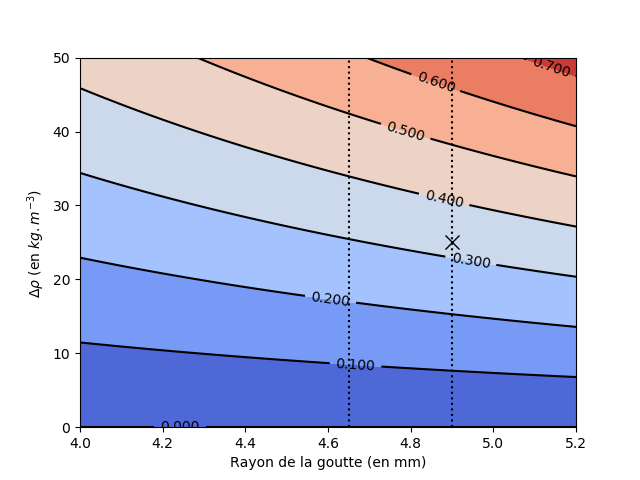
\includegraphics[width=0.7\linewidth]{figure/contour_bond}
	\caption[Valeur du nombre de Bond en fonction de la différence de densité et de la tension de surface entre les phases]{Valeur du nombre de Bond en fonction de la différence de densité entre les phases et le rayon de la goutte, le marqueur représente l'état initial}
	\label{fig:contourbond}
\end{figure}
Il est alors possible, dans notre cas, de discuter de la sphéricité de la goutte au vu de la valeur ici $Bo = 0.32$
